% !TEX root = ../my-thesis.tex
%
\chapter{Appendix}
\label{sec:appendix}
\section{Probability Distributions and the Exponential Family}
\subsection{The Exponential Family}
In statistics and probability theory, the \textit{exponential family} is a parametric set of probability distributions of a specific form. The distribution of a random variable $\pmb{y}$ belongs to the exponential family if the discrete or continuous density with respect to a $\sigma$-finite measure of $\pmb{y}$ has the form
\begin{equation}
    f(\pmb{y}|\pmb{\theta}, \lambda)=\exp\left(\frac{\pmb{y}^T\pmb{\theta} - b(\pmb{\theta})}{\lambda}+c(\pmb{y},\lambda) \right),
\end{equation}
with $c(\pmb{y},\lambda)\geq 0$. 
$\pmb{\theta}\in\Theta\subset\mathbb{R}^q$ is the \textit{natural} or \textit{canonical} parameter of the exponential family, while $\lambda > 0$ is a \textit{dispersion} or \textit{nuisance} parameter \autocite[][]{holland1981exponential}. The natural parameter space $\Theta$ is the set of all $\pmb{\theta}$ satisfying
\begin{equation}
    0<\int\exp\left(\left(\pmb{y}^T\pmb{\theta} - b(\pmb{\theta})\right)/\lambda+c(\pmb{y},\lambda) \right)d\pmb{y}< \infty
\end{equation} Moreover, $b(\pmb{\theta})$ is a twice differentiable  function and all moments of $\pmb{y}$ exist. Specifically, 
\begin{alignat}{3}
    \mathbb{E}_{\pmb{\theta}}(\pmb{y}) &= \mu(\pmb{\theta}) =& \frac{\partial b(\pmb{\theta})}{\partial\pmb{\theta}} \\
    \hbox{Cov}_{\pmb{\theta}}(\pmb{y}) &= \pmb{\Sigma}(\pmb{\theta}) =& \lambda\frac{\partial^2b(\pmb{\theta})}{\partial\pmb{\theta}\partial\pmb{\theta}^T}.
\end{alignat}
The covariance matrix $\pmb{\Sigma}(\pmb{\theta})$ is positive definite in $\Theta^0$, therefore $\mu:\Theta^0\rightarrow  M = \mu\left(\Theta^0\right)$ is injective. By substituting the inverse function $\pmb{\theta}(\mu)$ into $\frac{\partial^2b(\pmb{\theta})}{\partial\pmb{\theta}\partial\pmb{\theta}^T}$, the variance function 
\begin{equation}
    v(\mu)=\frac{\partial^2b(\pmb{\theta}(\mu))}{\partial\pmb{\theta}\partial\pmb{\theta}^T}
\end{equation}
is given and the covariance can be written as
\begin{equation}
    \hbox{Cov}_{\pmb{\theta}}(\pmb{y}) = \lambda v(\mu).
\end{equation}
Important members of the exponential family are the normal, binomial, Poisson, gamma and multivariate normal distribution \autocite[][433]{fahrmeir2013multivariate}.
\subsection{The Normal Distribution}
The normal distribution is an important type of continuous probability distribution in stochastics. The special significance of the normal distribution is based, among other things, on the central limit theorem, according to which distributions that result from the additive combination of a large number of independent influences are approximately normally distributed under weak conditions. \\
The density is given by
\begin{equation}
    f\left(x|\mu,\sigma\right)=\frac{1}{\sigma\sqrt{2\pi}}\exp\left(-\frac{1}{2}\left(\frac{\pmb{x}-\mu}{\sigma}\right)^2\right).
\end{equation}
The first two moments of the distribution are given by
\begin{align}
    \mathbb{E}\left[X\right] &= \mu \\
    \hbox{Var}\left[X\right] &= \sigma^2.
\end{align}
The graph of this density function has a "bell-shaped form" and is symmetrical with $\mu$ as the centre of symmetry \autocite[][83-85]{fahrmeir2016statistik}.
\subsection{The Multivariate Normal Distribution}
The density of a normally distributed random variable $\pmb{y}=\left(y_1,...,y_n\right)^T, n<\infty$ with mean vector $\pmb{\mu}$ ($n\times1$) and SPD covariance matrix $\pmb{\Sigma}$ ($n\times n$) is
\begin{equation}
    \pi\left(\pmb{y}\right)=\left(2\pi\right)^{-n/2}|\pmb{\Sigma}|^{-1/2}\exp\left(-\frac{1}{2}\left(\pmb{y}-\pmb{\mu}\right)^T\pmb{\Sigma}^{-1}\left(\pmb{y}-\pmb{\mu}\right)\right),\hspace{5pt}\pmb{y}\in\mathbb{R}^n
\end{equation}
Here, $\mu_i=\mathbb{E}\left[y_i\right]$, $ \Sigma_{ij}=\hbox{Cov}\left(y_i,y_j\right)$, $ \Sigma_{ii}=\hbox{Var}\left(y_i\right) > 0$ and $\hbox{Corr}\left(y_i,y_j\right)=\Sigma_{ij}/\left(\Sigma_{ii}\Sigma_{jj}\right)^{1/2}$. This is written as $\pmb{y}\sim\mathcal{N}\left(\pmb{\mu},\pmb{\Sigma}\right)$. For $n=1$, $\mu=0$ and $\Sigma_{11}=1$ the standard normal distribution is obtained. \\
$\pmb{y}$ is now split up into $\pmb{y}=\left(\pmb{y}_{\pmb{A}}^T,\pmb{y}_{\pmb{B}}^T\right)$ and $\pmb{\mu}$ and $\pmb{\Sigma}$ are divided accordingly:
\begin{equation*}
    \pmb{\mu} = \begin{pmatrix}\pmb{\mu}_{\pmb{A}} \\ \pmb{\mu}_{\pmb{B}}\end{pmatrix} \hspace{20pt}\hbox{ and }\hspace{20pt} \pmb{\Sigma}=\begin{pmatrix}\pmb{\Sigma}_{\pmb{AA}} & \pmb{\Sigma}_{\pmb{AB}}\\\pmb{\Sigma}_{\pmb{BA}} & \pmb{\Sigma}_{\pmb{BB}}\end{pmatrix}.
\end{equation*}
Some basic properties of the multivariate normal distribution are the following.
\begin{itemize}
    \item[1.] $\pmb{y}_{\pmb{A}}\sim\mathcal{N}\left(\pmb{\mu}_{\pmb{A}}, \pmb{\Sigma}_{\pmb{AA}}\right)$.
    \item[2.] $\pmb{\Sigma}_{\pmb{AB}}=\pmb{0}$ precisely when $\pmb{y}_{\pmb{A}}$ and $\pmb{y}_{\pmb{B}}$ are independent.
    \item[3.] The conditional distribution $\pi\left(\pmb{y}_{\pmb{A}}|\pmb{y}_{\pmb{B}}\right)$ is $\mathcal{N}\left(\pmb{\mu}_{\pmb{A}|\pmb{B}}, \pmb{\Sigma}_{\pmb{A}|\pmb{B}}\right)$, where
    \begin{align*}
        \pmb{\mu}_{\pmb{A}|\pmb{B}} &= \pmb{\mu}_{\pmb{A}}+\pmb{\Sigma}_{\pmb{AB}}\pmb{\Sigma}_{\pmb{BB}}^{-1}\left(\pmb{y}_{\pmb{B}}-\pmb{\mu}_{\pmb{B}}\right) \hbox{ and} \\
        \pmb{\Sigma}_{\pmb{A}|\pmb{B}} &= \pmb{\Sigma}_{\pmb{AA}}-\pmb{\Sigma}_{\pmb{AB}}\pmb{\Sigma}_{\pmb{BB}}^{-1}\pmb{\Sigma}_{\pmb{BA}}.
    \end{align*}
    \item[4.] If $\pmb{y}\sim\mathcal{N}\left(\pmb{\mu}, \pmb{\Sigma}\right)$ and $\pmb{y}'\sim\mathcal{N}\left(\pmb{\mu'}, \pmb{\Sigma'}\right)$ are independent, 
    \item[]then $\pmb{y}+\pmb{y'}\sim\mathcal{N}\left(\pmb{\mu}+ \pmb{\mu'}, \pmb{\Sigma}+ \pmb{\Sigma'}\right)$ \autocite[][19--20]{rue2005gaussian}.
\end{itemize}
\subsection{The Poisson Distribution}
The Poisson distribution is a discrete probability distribution that can be used to model the number of events that occur independently of each other at a constant mean rate in a fixed time interval or spatial area. \\
The density is given by
\begin{equation}
    f\left(k\right)=\mathbb{P}\left(X=k\right)=\begin{cases}
    \frac{\lambda^k}{k!}\exp\left(-\lambda\right) & \hbox{for }x\in\left\lbrace0,1,...\right\rbrace \\
    0 & \hbox{else}
    \end{cases}
\end{equation}
with $\lambda$ representing the expected value of $X$.  \\
The first two moments of the distribution are given by
\begin{align}
    \mathbb{E}\left[X\right] &= \lambda \label{eq:poisson_exp}\\
    \hbox{Var}\left[X\right] &= \lambda \label{eq:poisson_var}.
\end{align}
For $\lambda\geq10$ the distribution becomes approximately symmetrical and can thus be approximated by a normal distribution \autocite[][243]{fahrmeir2016statistik}. \clearpage
\subsection{The Negative Binomial Distribution}
The negative binomial distribution is a univariate probability distribution that belongs to the discrete probability distributions. It models the number of trials required to achieve a given number of successes in a Bernoulli process. \\
The density is given by
\begin{equation}
    f\left(k,r,p\right)=\mathbb{P}\left(X=k\right)=\begin{pmatrix} k+r-1\\r-1\end{pmatrix}\left(1-p\right)^kp^r,
\end{equation}
with $r$ the number of successes, $k$ the number of failures, and $p$ the probability of success. \\
The first two moments of the distribution are given by
\begin{align}
    \mathbb{E}\left[X\right] &= \frac{pr}{1-p} \\
    \hbox{Var}\left[X\right] &= \frac{pr}{\left(1-p\right)^2}.
\end{align} 
For large values of $r$, the negative binomial distribution can be approximated by a normal distribution
\autocite[][]{haldane1941fitting}.
\clearpage
\section{Symmetric Positive Definite Matrices}
An $n \times n$ matrix $\pmb{A}$ is \textit{positive definite} exactly if
\begin{equation*}
    \pmb{x}^T\pmb{A}\pmb{x}>0,\hspace{20pt}\forall\pmb{x}\neq\pmb{0}.
\end{equation*}
If $\pmb{A}$ is also symmetric, it is called a symmetric positive definite (SPD) matrix. Only SPD matrices are considered and sometimes the notation '$\pmb{A}>0$' is used for an SPD matrix $\pmb{A}$. \\
An SPD matrix $\pmb{A}$ has some of the following properties.
\begin{itemize}
    \item[1.] $\hbox{rank}\left(\pmb{A}\right)=n$.
    \item[2.] $|\pmb{A}|>0$.
    \item[3.] $A_{ii}>0$.
    \item[4.] $A_{ii}A_{jj}-A_{ij}^2>0$, for $i\neq j$.
    \item[5.] $A_{ii} + A_{jj}-2|A_{ij}|>0$ for $i\neq j$.
    \item[6.] $\max A_{ii}>\max_{i\neq j}|A_{ij}|$.
    \item[7.] $\pmb{A}^{-1}$ is SPD.
    \item[8.] All principal submatrices of $\pmb{A}$ are SPD.
\end{itemize}
If $\pmb{A}$ and $\pmb{B}$ are SPD, $\pmb{A}+\pmb{B}$ is SPD, but the reverse is generally not true. Additionally, if $\pmb{AB}=\pmb{BA}$, $\pmb{AB}$ is SPD. \\
The following conditions are all sufficient and necessary for a symmetric matrix $\pmb{A}$ to be SPD:
\begin{itemize}
    \item[1.] All eigenvalues $\lambda_1,...,\lambda_n$ of $\pmb{A}$ are strictly positive.
    \item[2.] There exists such a matrix $\pmb{C}$ that $\pmb{A}=\pmb{CC}^T$. If $\pmb{C}$ is lower triangular, it is called the \textit{Cholesky triangle} of $\pmb{A}$.
    \item[3.] All leading principal submatrices have strictly positive determinants.
\end{itemize}    
A sufficient, but not necessary condition for a (symmetrical) matrix to be SPD is the criterion of \textit{diagonal dominance}:
    \begin{equation*}
        A_{ii}-\sum_{j:j\neq i}|A_{ij}|>0,\hspace{20pt}\forall i.
    \end{equation*}
    A $n\times n$ matrix $\pmb{A}$ is called a \textit{symmetric positive semidefinite} (SPSD) matrix. An SPSD matrix $\pmb{A}$ is sometimes denoted '$\pmb{A}\geq0$' \autocite[][18--19]{rue2005gaussian}.
\clearpage
\section{Example: PC Prior for the Precision}
A PC prior can be used to adjust the smoothness of a spatial field in an intuitive way by specifying such a prior for the precision $\tau$. This makes it possible to adjust the smoothness of the spatial field in an intuitive way. In this case, the penalized complexity prior is defined by the upper limit $\sigma_0$. Equation~\ref{eq:pcprior} therefore looks like this,
\begin{equation}\label{pcprec}
    \mathbb{P}\left(\sigma > \sigma_0\right)=\alpha.
\end{equation}
The actual expression of the prior is given by
\begin{equation}\label{eq:pc_prior_prec}
    \pi\left(\tau\right)=\frac{\lambda}{2}\tau^{-3/2}\exp\left(-\lambda\tau^{-1/2}\right),\hspace{20pt}\tau>0
\end{equation}
and is a type-2-Gumbel distribution. \\
The prior for $\tau$ corresponds to an exponential distribution with rate $\lambda$ for the standard deviation. $\lambda$ quantifies the size of the penalty for deviation from the base model and is increased with higher values for it. Here, $\lambda=\frac{-\log\left(\alpha\right)}{\sigma_0}$ \autocite[][]{sorbye2017penalised}.
\clearpage
\section{Goodness-of-Fit indicators}\label{sec:performance}
The goodness of fit indicates "how well" an estimated model can explain a set of observations. Measures of goodness of fit allow a statement to be made about the discrepancy between the theoretical values of the random variables under investigation, which are expected or predicted on the basis of the model, and the values actually measured. \\
The goodness of fit of a model to available data can be assessed with the help of statistical tests or suitable ratios.
\subsection{The Akaike Information Criterion}
The historically oldest criterion was proposed in 1973 by Hirotsugu Akaike (1927-2009) as an information criterion and is known today as the Akaike information criterion (AIC). The AIC is one of the most frequently used criteria for model selection in the context of likelihood-based inference.  \\
Let the population contain the distribution of a variable with unknown density function $p$. The maximum likelihood estimation assumes a known distribution with an unknown parameter $\theta$, hence the density function can be written as $q\left(\theta\right)$. The Kullback-Leibler divergence is used as a distance measure between $p$ and $q\left(\widehat{\theta}\right)$ with $\widehat{\theta}$ the estimated parameter from the maximum likelihood estimation. The better the maximum likelihood model, the small the Kullback-Leibler divergence $D\left(P||Q\right)$. \\
For a maximum likelihood model with a $p$-dimensional parameter vector $\widehat{\pmb{\theta}}$, the Akaike information criterion is defined as
\begin{equation}
    \hbox{AIC}=-2l\left(\widehat{\pmb{\theta}}_{ML}\right)+2p,
\end{equation}
with $l$ the log-likelihood function \autocite[][]{akaike1974new}.
\subsection{The Deviance Information Criterion}
In statistics, the deviance information criterion, or DIC for short, is a measure (criterion) for the prediction error of a model.
This measure is an information criterion and belongs to the environment of the Bayesian method for model comparisons. The smaller the deviance information criterion, the better the model fit. The deviance information criterion can be regarded as the Bayesian equivalent of the Akaike information criterion. \\
The deviance is defined as 
\begin{equation}
    D\left(\pmb{\theta}\right)=-2\log\left(l\left(\pmb{y}|\pmb{\theta}\right)\right)+C,
\end{equation}
with $\pmb{y}$ the data, $\pmb{\theta}$ the unknown parameters of the model and $l$ the likelihood function. $C$ is a constant that cancels out in all calculations that compare different models and therefore it does not need to be known \autocite[][]{nelder1972generalized}. \\
The DIC is given by
\begin{equation}
    \hbox{DIC}=D\left(\overline{\pmb{\theta}}\right)+2p_D,
\end{equation}
with
\begin{equation}
    p_D=\overline{D\left(\pmb{\theta}\right)}-D\left(\overline{\pmb{\theta}}\right),
\end{equation}
where $\overline{\pmb{\theta}}$ is the expected value of $\pmb{\theta}$ \autocite[][]{spiegelhalter2014deviance}.
\subsection{The Watanabe-Akaike Information Criterion}
The Watanabe-Akaike information criterion (WAIC) is the generalized AIC onto singular statistical models.
The WAIC is given by
\begin{equation}
    \hbox{WAIC} = -2\hbox{LLPD}+2p_{\hbox{WAIC}},
\end{equation}
with the log pointwise predictive density (LLPD) given by
\begin{equation}
    \hbox{LLPD} = \sum_{i=1}^n\log\left(\int \pi\left(y_i|\pmb{\theta}\right)\pi_{\hbox{post}}\left(\pmb{\theta}\right)\right)d\pmb{\theta}.
\end{equation}
LLPD can be seen as the Bayesian analogue of $l\left(\widehat{\pmb{\theta}}_{ML}\right)$ in the calculation of the AIC.\\
The penalty term of the WAIC is fully Bayesian and given by
\begin{equation}
    p_{\hbox{WAIC}}=\sum_{i=1}^n\hbox{Var}_{\hbox{post}}\left(\log\left(\pi\left(y_i|\pmb{\theta}\right)\right)\right),
\end{equation}
where the term represents the variance of the individual terms in the LLPD over all data points \autocite[][]{watanabe2010asymptotic, yong2018loo}. \clearpage
\subsection{The Conditional Predictive Ordinate}
The conditional predictive ordinate (CPO) is a Bayesian diagnostic that can be used to detect surprising observations. It is often used in the context of univariate sampling, the multivariate normal distribution and regression models. \\
The conditional predictive ordinate is given by
\begin{equation}
    \hbox{CPO} = \pi\left(y_i|\pmb{y}_{-i}\right)
\end{equation}
with $\pmb{y}$ the data, $\pmb{y}_{-i}$ the data without the $i$-th observation, and $\pi\left(\cdot|\pmb{y}_{-i}\right)$ the predictive distribution of a new observation at $\pmb{y}_{-i}$. Low values of CPO are an indication that $y_i$ is surprising given prior knowledge and the other observations \autocite[][]{pettit1990conditional, cox1980discussion}.
\subsection{The Mean Absolute Error}
The mean absolute error (MAE) is a statistical quantity that can be used to determine the accuracy of predictions. Let $\widehat{x}_i$ be the predicted value and $x_i$ the true value, then
\begin{equation}
    \frac{1}{n}\sum_{i=1}^n\left|\widehat{x}_i-x_i\right|
\end{equation}
\autocite[][]{willmott2005advantages}.
\clearpage
\section{The Variance Inflation Factor}\label{sec:vif}
The Variance Inflation Factor ($\hbox{VIF}$) is a measurement that can be used to avoid multicollinearity between covariates. The $\hbox{VIF}$ quantifies the severity of multicollinearity in a generalized linear model. It provides an index that measures the extent to which the variance of an estimated regression coefficient is increased due to collinearity. \\
For $p-1$ independent variables, 
\begin{equation}
    \hbox{VIF}_i = \frac{1}{1-R^2},\hspace{20pt}i=1,...,p-1,
\end{equation}
with $R^2$ the coefficient of determination. In most literature, a value of at least 5 is suggested as too high and is therefore used as the threshold in this work \autocite[][]{craney2002model}.
\clearpage
\section{Moments}
\subsection{Skewness}
Skewness is a statistical indicator that describes the type and strength of the asymmetry of a probability distribution. It shows whether and how strongly the distribution is skewed to the right (right-skewed, left-skewed, negative skewness) or to the left (left-skewed, right-skewed, positive skewness). Any non-symmetrical distribution is called skewed. \\
The skewness of a random variable $X$ is the third standardized moment, defined as
\begin{equation}\label{eq:skewness}
    \hbox{Skew}[X]=\mathbb{E}\left[\left(\frac{X-\mu}{\sigma}\right)^3\right] = \frac{\mathbb{E}\left[\left(X-\mu\right)^3\right]}{\left(\mathbb{E}\left[\left(X-\mu\right)^{3/2}\right]\right)^2}=\frac{\mu_3}{\sigma^3},
\end{equation}
with $\mu_3$ the third central moment and $\sigma$ the standard deviation \autocite[][]{doane2011measuring, wilkins1944note}.
\subsection{Kurtosis}
Kurtosis is a measure of the slope of a probability distribution of a random variable. Distributions with low kurtosis scatter relatively evenly; for distributions with high kurtosis, the scatter results more from extreme but rare events. \\
The kurtosis of a random variable $X$ is the fourth standardized moment, defined as
\begin{equation}\label{eq:kurtosis}
    \hbox{Kurt}[X]=\mathbb{E}\left[\left(\frac{X-\mu}{\sigma}\right)^4\right] = \frac{\mathbb{E}\left[\left(X-\mu\right)^4\right]}{\left(\mathbb{E}\left[\left(X-\mu\right)^2\right]\right)^2}=\frac{\mu_4}{\sigma^4},
\end{equation}
with $\mu_4$ the fourth central moment and $\sigma$ the standard deviation \autocite[][]{decarlo1997meaning, wilkins1944note}.
\clearpage
\section{Distribution Fits}
\subsection{Distribution Fits for Germany}
\subsubsection{Fits for the Non-Temporal Models}
\begin{figure}[H]
    \centering
    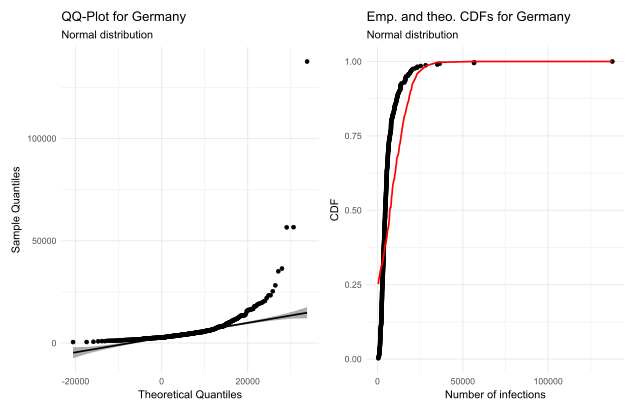
\includegraphics[width = 0.9\textwidth]{fit_normal_germany.png}
    \caption{A normal fit to the number of cases in German municipalities}
    \label{fitNormalGermany}
\end{figure}
\begin{figure}[H]
    \centering
    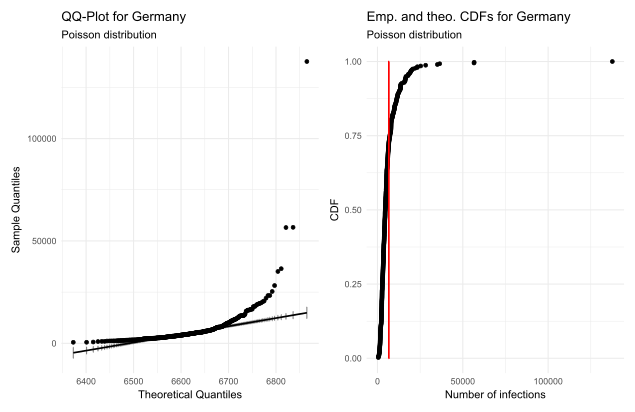
\includegraphics[width = 0.9\textwidth]{fit_poisson_germany.png}
    \caption{A Poisson fit to the number of cases in German municipalities}
    \label{fitPoissonGermany}
\end{figure}
\clearpage
\subsubsection{Fits for the Temporal Models}\label{sec:temp_fit_germany}
\begin{figure}[H]
  \centering
  \includegraphics[width = 0.9\textwidth]{fit_poisson_germany_ts.png}
  \caption{A Poisson fit to the number of cases in German municipalities}
  \label{fitPoissonGermany_ts}
\end{figure}
\subsection{Distribution Fits for Norway}
\subsubsection{Fits for the Non-Temporal Models}\label{sec:temp_fit_norway}
\begin{figure}[H]
    \centering
    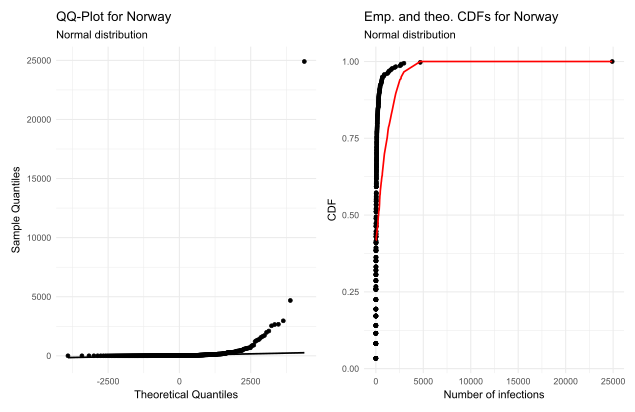
\includegraphics[width = 0.9\textwidth]{fit_normal_norway.png}
    \caption{A normal fit to the number of cases in Norwegian municipalities}
    \label{fitNormalNorway}
\end{figure}
\clearpage
\begin{figure}[H]
    \centering
    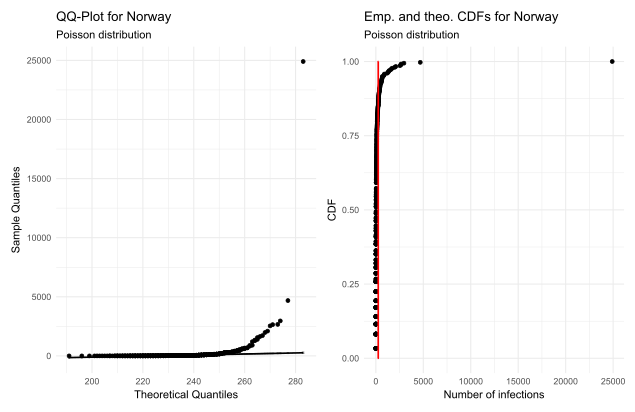
\includegraphics[width = 0.9\textwidth]{fit_poisson_norway.png}
    \caption{A Poisson fit to the number of cases in Norwegian municipalities}
    \label{fitPoissonNorway}
\end{figure}
\subsubsection{Fits for the Temporal Models}
\begin{figure}[H]
  \centering
  \includegraphics[width = 0.9\textwidth]{fit_nbinom_norway_ts.png}
  \caption{A negative binomial fit to the number of cases in Norwegian municipalities}
  \label{fitNegbinomNorway_ts}
\end{figure}
\clearpage
\begin{figure}[H]
  \centering
  \includegraphics[width = 0.9\textwidth]{fit_normal_norway_ts.png}
  \caption{A normal fit to the number of cases in Norwegian municipalities}
  \label{fitNormalNorway_ts}
\end{figure}
\begin{figure}[H]
  \centering
  \includegraphics[width = 0.9\textwidth]{fit_poisson_norway_ts.png}
  \caption{A Poisson fit to the number of cases in Norwegian municipalities}
  \label{fitPoissonNorway_ts}
\end{figure}
\clearpage
\begin{figure}[H]
  \centering
  \includegraphics[width = 0.9\textwidth]{distrfit_norway_ts.png}
  \caption{Histogram for the number of cases in Norwegian municipalities with a normal and a negative binomial distribution overlayed.}
  \label{fitDistrNorway_ts}
\end{figure}
\clearpage
\section{Choice of Hyperpriors for Germany}
\begin{figure}[H]
    \centering
    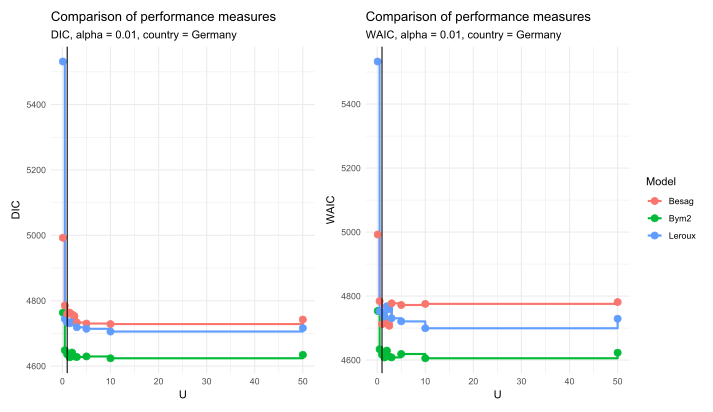
\includegraphics[width = \textwidth]{comparison_1_germany.png}
    \caption{Values of the DIC and the WAIC when changing the value for $\sigma_0$. The black line highlights the values for $\sigma_0$ = 1.}
    \label{comparison_germany_1}
\end{figure}
\begin{figure}[H]
    \centering
    \includegraphics[width = \textwidth]{mae_germany.png}
    \caption{Values of the MAE when changing the value for $\sigma_0$. The black line highlights the values for $\sigma_0$ = 1.}
    \label{comparison_germany_2}
\end{figure}

\begin{figure}[H]
    \centering
    \includegraphics[width = \textwidth]{spatial_field_germany_1.png}
    \caption{Spatial field for a Besag model and a Leroux model.}
    \label{comparison_germany_6}
\end{figure}
\begin{figure}[H]
    \centering
    \includegraphics[width = \textwidth]{spatial_field_germany_2.png}
    \caption{Spatial fields for a BYM2 model.}
    \label{comparison_germany_7}
\end{figure}
\clearpage
% \section{Code Examples}
% \subsection{Specifying the Different Types of Models}
% \begin{lstlisting}[caption={Specifying different models in INLA.}, label={codeModels}, language=R]
% # set the seed
% set.seed(420)
% # draw a sample
% test <- sample(
%     seq_len(nrow(newest_numbers)),
%     size = floor(0.2 * nrow(newest_numbers))
%   )
% # get the number of infections for the test data
% test_value <- newest_numbers$value[test]
% # set the number of infections to NA in the train data
% newest_numbers$value[test] <- NA
% # define the link function
% link <- rep(NA, nrow(newest_numbers))
% link[which(is.na(newest_numbers$value))] <- 1
% # for the temporal model every 5th day is taken
% germany <- germany[
%   germany$Date %in% seq(
%     from = min(germany$Date),
%     to = max(germany$Date),
%     by = 5
%   ),
% ]
% # draw a sample
% test_temporal <- sample(
%   seq_len(nrow(germany)),
%   size = floor(0.2 * nrow(germany))
% )
% test_value_temporal <- germany$value[test_temporal]
% germany$value[test_temporal] <- NA
% link_temporal <- rep(NA, nrow(germany))
% link_temporal[which(is.na(germany$value))] <- 1
% # define the penalised prior
% prior_1 <- list(
%   prec = list(
%     prior = "pc.prec",
%     param = c(1, 0.01)
%   )
% )
% # create the neighbordhood matrix
% nb <- poly2nb(newest_numbers)
% # save the matrix
% nb2INLA("maps/map.adj", nb)
% g <- inla.read.graph(filename = "maps/map.adj")
% # define the C matrix for the Leroux model
% Q <- Diagonal(x = sapply(nb, length))
% for (i in 2:nrow(newest_numbers)) {
%   Q[i - 1, i] <- -1
%   Q[i, i - 1] <- -1
% }

% C <- Diagonal(x = 1, n = nrow(newest_numbers)) - Q
% # formula for the model without the spatial component
% formula_1 <- value ~
%   pop_dens + urb_dens + sex + trade_tax + SPD + Gruene + FDP +
%   die_linke + clinic + place_of_worship + nursing_home +
%   aerodrome + platform + office + marketplace + higher_education
% # formula for the besag model
% formula_2 <- value ~
%   pop_dens + urb_dens + sex + trade_tax + SPD + Gruene + FDP +
%   die_linke + clinic + place_of_worship + nursing_home +
%   aerodrome + platform + office + marketplace + higher_education +
%   f(idarea_1, model = "besagproper", graph = g, hyper = prior_1)
% # formula for the bym2 model
% formula_3 <- value ~
%   pop_dens + urb_dens + sex + trade_tax + SPD + Gruene + FDP +
%   die_linke + clinic + place_of_worship + nursing_home +
%   aerodrome + platform + office + marketplace + higher_education +
%   f(
%     idarea_1, model = "bym2", graph = g,
%     scale.model = TRUE, hyper = prior_1
%   )
% # formula for the leroux model
% formula_4 <- value ~
%   pop_dens + urb_dens + sex + trade_tax + SPD + Gruene + FDP +
%   die_linke + clinic + place_of_worship + nursing_home +
%   aerodrome + platform + office + marketplace + higher_education +
%   f(idarea_1, model = "generic1", Cmatrix = C, hyper = prior_1)
% # formula for the temporal bym2 model
% formula_5 <- value ~
%   pop_dens + urb_dens + sex + trade_tax + SPD + Gruene + FDP +
%   die_linke + clinic + place_of_worship + nursing_home +
%   aerodrome + platform + office + marketplace + higher_education +
%   f(
%     idarea_1, model = "bym2", graph = g,
%     scale.model = TRUE, hyper = prior_1
%   ) +
%   f(id_date_1, model = "rw2", hyper = prior_1)
% # compute the models
% # for the non-temporal models the code looks like this
% res_1 <- inla(
%   formula_1,
%   family = "nbinomial",
%   data = newest_numbers,
%   E = expected_count,
%   control.predictor = list(
%     compute = TRUE,
%     link = link
%   ),
%   Ntrials = newest_numbers$population,
%   control.compute = list(dic = TRUE, waic = TRUE, cpo = TRUE)
% )
% # for the temporal models the code looks like this
% res_5 <- inla(
%   formula_5,
%   family = "nbinomial",
%   data = germany,
%   E = expected_count,
%   control.predictor = list(
%     compute = TRUE,
%     link = link_temporal
%   ),
%   Ntrials = germany$population,
%   control.compute = list(dic = TRUE, waic = TRUE, cpo = TRUE)
% )
% \end{lstlisting}
% \subsection{Making Predictions for the Test Data}
% \begin{lstlisting}[caption={The code for making predictions in INLA.}, label={codePrediction}, language=R]
% \end{lstlisting}
% \subsection{Calculating the Posterior Mean}
% \begin{lstlisting}[caption={Calculating the posterior mean of a coefficent.}, label={codePosteriorMean}, language=R]
% inla.emarginal(
%       exp,
%       res_1$marginals.fixed$`(Intercept)`
% )
% \end{lstlisting}
% \subsection{Calculating a Credibility Interval}
% \begin{lstlisting}[caption={Extracting the credibility interval for a coefficient}, label={codeCredibility}, language=R]
% inla.qmarginal(
%       c(0.025, 0.975),
%       inla.tmarginal(
%         exp,
%         res_1$marginals.fixed$`(Intercept)`
%       )
% )
% \end{lstlisting}
% \subsection{Calculating the Temporal Trend}
% \begin{lstlisting}[caption={Calculating the Temporal Trend of a Model}, label={codeTemporal}, language=R]
% temporal_car <- lapply(
%   res_5$marginals.random$id_date_1,
%   function(x) {
%     marg <- inla.tmarginal(
%       function(y) exp(y),
%       x
%     )
%     inla.emarginal(mean, marg)
%   }
% )
% \end{lstlisting}

\clearpage
\section{OpenStreetMap Key-Value Pairs}\label{sec:kv}
\begin{table}[H]
\caption{A list of all the key-value pairs used to query OpenStreetMap, except the ones used for residential buildings \label{OSM}}
\begin{tabular}{l l l}
\toprule
\textbf{Key} & \textbf{Value} & \textbf{Description} \\
\midrule
\multirow{21}{*}{amenity} & cinema & A place where films are shown \\
& \multirow{2}{*}{clinic} & A medium-sized medical facility \\
& & or health centre. \\
& \multirow{2}{*}{college} & Campus or buildings of an institute \\
& & of Further Education \\
& dentist & A dentist practice / surgery \\
& doctors &  A doctor's practice / surgery \\
& \multirow{2}{*}{hospital} & A hospital providing in-patient \\
& & medical treatment \\
& kindergarten & For children too young for a regular school \\
& \multirow{2}{*}{marketplace} & A marketplace where goods and services \\
& & are traded daily or weekly \\
& nightclub & A place to drink and dance \\
& nursing\_home & A home for disabled or elderly persons \\
& place\_of\_worship &  A church, mosque, or temple, etc. \\
& restaurant & A restaurant \\
& \multirow{2}{*}{school} & School and grounds - primary, middle \\
& & and secondary schools \\
& theatre & A theatre or opera house \\
& \multirow{2}{*}{university} & An university campus: an institute \\
& & of higher education\\
\midrule 
\multirow{3}{*}{building} & office & An office building \\
& \multirow{2}{*}{retail} & A building primarily used for selling goods \\
& & that are sold to the public \\
\midrule
\multirow{3}{*}{leisure} & fitness\_centre & Fitness centre, health club or gym \\
& \multirow{2}{*}{sports\_centre} & Facility where sports take place within \\
& & an enclosed area \\
\midrule
public\_transport & platform & Public transport platforms \\
\midrule
\multirow{7}{*}{shop} & bakery & Shop focused on selling bread	\\
& \multirow{2}{*}{chemist} & Shop focused on selling articles of personal \\
& & hygiene, cosmetics, household products \\
& \multirow{2}{*}{convenience} & A small local shop carrying a small subset \\
& & of the items you would find in a supermarket	\\
& hairdresser & Here you can get your hair cut, coloured \\
& supermarket & A large store with groceries and other items \\
\bottomrule
\end{tabular}
\end{table}
\begin{table}[H]
\caption{A list of all the key-value pairs used to query OpenStreetMap for residential buildings \label{OSM_2}}
\begin{tabular}{l l l}
\toprule
\textbf{Key} & \textbf{Value} & \textbf{Description} \\
\midrule
\multirow{21}{*}{building} & \multirow{2}{*}{apartments} & A building arranged into individual dwellings, \\
& & often on separate floors \\
& bungalow & A single-storey detached small house \\
& cabin & A small, roughly built house \\
& detached & A free-standing residential building \\
& \multirow{2}{*}{dormitory} & A shared building intended for college/\\
& & university students \\
& farm & A residential building on a farm \\
& \multirow{2}{*}{ger} & A permanent or seasonal round yurt or \\
& & ger used as dwelling \\
& \multirow{2}{*}{hotel} & A building designed with separate rooms \\
& & available for overnight accommodation \\
& house & A dwelling unit inhabited by a single household \\
& houseboat & A boat used primarily as a home\\
& residential & A building used primarily for residential purposes \\
& \multirow{2}{*}{semidetached\_house} & A residential house that shares a common wall \\
& & with another on one side \\
& \multirow{2}{*}{static caravan} & A mobile home (semi)permanently left \\
& & on a single site \\
& terrace & A linear row of residential dwellings \\
\bottomrule
\end{tabular}
\end{table}
\clearpage
\subsection*{Combination of Key-Value Pairs}
The following table shows which key-value pairs were combined, due to their similarity.
\begin{table}[H]
\caption{A list of all the key-value pairs that were combined to create variables \label{OSM_3}}
\begin{tabular}{l l l}
\toprule
\textbf{Key} & \textbf{Value} & \textbf{Variable} \\
\midrule
\multirow{3}{*}{amenity} & cinema & \multirow{3}{*}{Entertainment} \\
& nightclub \\
& theatre \\
\midrule
\multirow{3}{*}{amenity} & clinic & \multirow{3}{*}{Clinic} \\
& dentist \\
& doctors \\
\midrule
\multirow{2}{*}{amenity} & college & \multirow{2}{*}{Higher Education} \\
& university \\
\midrule
\multirow{2}{*}{leisure} & fitness\_centre & \multirow{2}{*}{Sports} \\
& sports\_centre \\
\midrule
\multirow{3}{*}{shop} & chemist & \multirow{3}{*}{Shop} \\
& convenience \\
& supermarket \\
\bottomrule
\end{tabular}
\end{table}
\clearpage
\section{Software Used}
All the analysis that was carried out was done so using the 4.1 version of the statistical software R \autocite[][]{baser}. The following packages were used as part of the analysis:
\begin{itemize}
    \item \texttt{covid19germany} \autocite[][]{covid19germany}
    \item \texttt{covidregionaldata} \autocite[][]{covidregionaldata}
    \item \texttt{data.table} \autocite[][]{data.table}
    \item \texttt{dashboardthemes} \autocite[][]{dashboardthemes}
    \item \texttt{dplyr} \autocite[][]{dplyr}
    \item \texttt{DT} \autocite[][]{DT}
    \item \texttt{eurostat} \autocite[][]{eurostat}
    \item \texttt{fitdistrplus} \autocite[][]{fitdistrplus}
    \item \texttt{furrr} \autocite[][]{furrr}
    \item \texttt{geosphere} \autocite[][]{geosphere}
    \item \texttt{ggplot2} \autocite[][]{ggplot2}
    \item \texttt{here} \autocite[][]{here}
    \item \texttt{highcharter} \autocite[][]{highcharter}
    \item \texttt{iml} \autocite[][]{iml}
    \item \texttt{INLA} \autocite[][]{INLA}
    \item \texttt{ISOcodes} \autocite[][]{ISOcodes}
    \item \texttt{LaCroixColoR} \autocite[][]{LaCroixColoR}
    \item \texttt{lwgeom} \autocite[][]{lwgeom}
    \item \texttt{latex2exp} \autocite[][]{latex2exp}
    \item \texttt{mapdeck} \autocite[][]{mapdeck}
    \item \texttt{MASS} \autocite[][]{MASS}
    \item \texttt{mlr} \autocite[][]{mlr}
    \item \texttt{osmdata} \autocite[][]{osmdata}
    \item \texttt{parallelMap} \autocite[][]{parallelMap}
    \item \texttt{patchwork} \autocite[][]{patchwork}
    \item \texttt{pbapply} \autocite[][]{pbapply}
    \item \texttt{qqplotr} \autocite[][]{qqplotr}
    \item \texttt{readr} \autocite[][]{readr}
    \item \texttt{regclass} \autocite[][]{regclass}
    \item \texttt{reshape2} \autocite[][]{reshape2}
    \item \texttt{rlist} \autocite[][]{rlist}
    \item \texttt{RSelenium} \autocite[][]{RSelenium}
    \item \texttt{sass} \autocite[][]{sass}
    \item \texttt{sf} \autocite[][]{sf}
    \item \texttt{shiny} \autocite[][]{shiny}
    \item \texttt{shinybusy} \autocite[][]{shinybusy}
    \item \texttt{shinydashboard} \autocite[][]{shinydashboard}
    \item \texttt{shinyWidgets} \autocite[][]{shinyWidgets}
    \item \texttt{SpatialEpi} \autocite[][]{SpatialEpi}
    \item \texttt{spdep} \autocite[][]{spdep}
    \item \texttt{stringr} \autocite[][]{stringr}
    \item \texttt{tibble} \autocite[][]{tibble}
    \item \texttt{units} \autocite[][]{units}
    \item \texttt{waiter} \autocite[][]{waiter}
\end{itemize}
All of the code used in this work is available through the following GitHub repository:
\begin{center}
    \href{https://github.com/nicoFhahn/masterthesis}{https://github.com/nicoFhahn/masterthesis}
\end{center}